\chapter{Введение}

\section{Цель работы}

Исследование влияния высокочастотного навязывания на линии передачи информации.

\begin{figure}
 \centering
 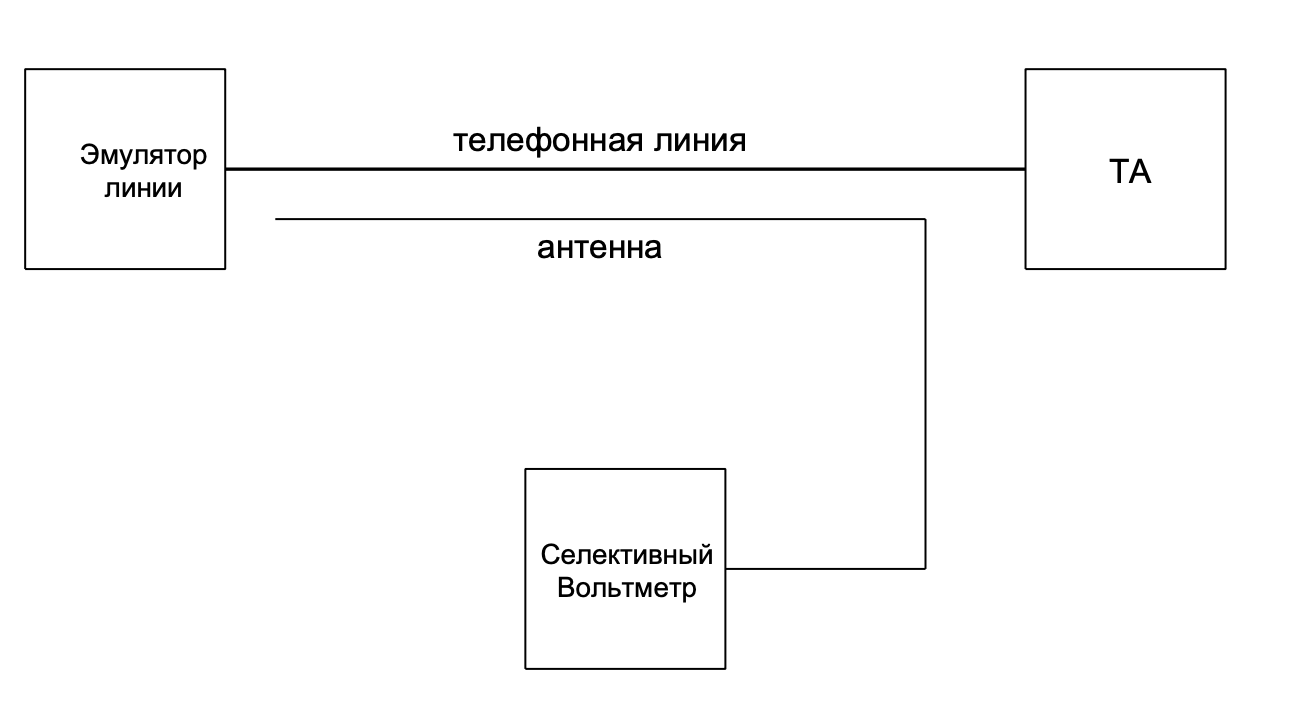
\includegraphics[width=.9\textwidth]{img/scheme.png}
 \caption{приципиальная схема лабораторной установки}
\end{figure}

\chapter{Ход работы}


\begin{table}[]
	\centering
	\begin{tabular}{|l|l|}
	\hline
	Частота, Гц & Уровень поля, мВ  \\ \hline
	10          & 12.5 \\ \hline
	20          & 12.5  \\ \hline
	30          & 12.5 \\ \hline
	40          & 12.5 \\ \hline
	50          & 12.5 \\ \hline
	60          & 12.5  \\ \hline
	70          & 12.5 \\ \hline
	80          & 12.5 \\ \hline
	90          & 12.5 \\ \hline
	100         & 12.5 \\ \hline
	110         & 12.5 \\ \hline
	120         & 12.5 \\ \hline
	130         & 12.5 \\ \hline
	140         & 12.5 \\ \hline
	150         & 12.5 \\ \hline
	160         & 12.5 \\ \hline
	170         & 12.5 \\ \hline
	180         & 12.5 \\ \hline
	190         & 12.5 \\ \hline
	200         & 15  \\ \hline
	210         & 12.5 \\ \hline
	220         & 15  \\ \hline
	230         & 15  \\ \hline
	240         & 17  \\ \hline
	250         & 17  \\ \hline
	\end{tabular}
	\caption{зависимость уровня поля от частоты}
	\label{tab:my-table}
	\end{table}


\begin{tikzpicture}
\begin{axis}[
title={Зависимость уровня поля от частоты диапазона},
xlabel={Частота, Гц},
ylabel={Уровень поля, мВ},
xmin=0, xmax=300,
ymin=10, ymax=20,
legend pos=north west,
ymajorgrids=true,
grid style=dashed,
]

\addplot[
color=blue,
mark=square,
]
coordinates {
(10, 12.5)(20, 12.5)(30, 12.5)(40, 12.5)(50, 12.5)(60, 12.5)(70, 12.5)(80, 12.5)(90, 12.5)(100, 12.5)(110, 12.5)(120, 12.5)(130, 12.5)(140, 12.5)(150, 12.5)(160, 12.5)(170, 12.5)(180, 12.5)(190, 12.5)(200, 15  )(210, 12.5)(220, 15  )(230, 15  )(240, 17  )(250, 17  )
};


\end{axis}
\end{tikzpicture}